% Options for packages loaded elsewhere
\PassOptionsToPackage{unicode}{hyperref}
\PassOptionsToPackage{hyphens}{url}
\PassOptionsToPackage{dvipsnames,svgnames,x11names}{xcolor}
%
\documentclass[
  10pt,
  dvipsnames,enabledeprecatedfontcommands]{scrartcl}
\usepackage{amsmath,amssymb}
\usepackage{lmodern}
\usepackage{iftex}
\ifPDFTeX
  \usepackage[T1]{fontenc}
  \usepackage[utf8]{inputenc}
  \usepackage{textcomp} % provide euro and other symbols
\else % if luatex or xetex
  \usepackage{unicode-math}
  \defaultfontfeatures{Scale=MatchLowercase}
  \defaultfontfeatures[\rmfamily]{Ligatures=TeX,Scale=1}
\fi
% Use upquote if available, for straight quotes in verbatim environments
\IfFileExists{upquote.sty}{\usepackage{upquote}}{}
\IfFileExists{microtype.sty}{% use microtype if available
  \usepackage[]{microtype}
  \UseMicrotypeSet[protrusion]{basicmath} % disable protrusion for tt fonts
}{}
\usepackage{xcolor}
\usepackage{graphicx}
\makeatletter
\def\maxwidth{\ifdim\Gin@nat@width>\linewidth\linewidth\else\Gin@nat@width\fi}
\def\maxheight{\ifdim\Gin@nat@height>\textheight\textheight\else\Gin@nat@height\fi}
\makeatother
% Scale images if necessary, so that they will not overflow the page
% margins by default, and it is still possible to overwrite the defaults
% using explicit options in \includegraphics[width, height, ...]{}
\setkeys{Gin}{width=\maxwidth,height=\maxheight,keepaspectratio}
% Set default figure placement to htbp
\makeatletter
\def\fps@figure{htbp}
\makeatother
\setlength{\emergencystretch}{3em} % prevent overfull lines
\providecommand{\tightlist}{%
  \setlength{\itemsep}{0pt}\setlength{\parskip}{0pt}}
\setcounter{secnumdepth}{5}
\newlength{\cslhangindent}
\setlength{\cslhangindent}{1.5em}
\newlength{\csllabelwidth}
\setlength{\csllabelwidth}{3em}
\newlength{\cslentryspacingunit} % times entry-spacing
\setlength{\cslentryspacingunit}{\parskip}
\newenvironment{CSLReferences}[2] % #1 hanging-ident, #2 entry spacing
 {% don't indent paragraphs
  \setlength{\parindent}{0pt}
  % turn on hanging indent if param 1 is 1
  \ifodd #1
  \let\oldpar\par
  \def\par{\hangindent=\cslhangindent\oldpar}
  \fi
  % set entry spacing
  \setlength{\parskip}{#2\cslentryspacingunit}
 }%
 {}
\usepackage{calc}
\newcommand{\CSLBlock}[1]{#1\hfill\break}
\newcommand{\CSLLeftMargin}[1]{\parbox[t]{\csllabelwidth}{#1}}
\newcommand{\CSLRightInline}[1]{\parbox[t]{\linewidth - \csllabelwidth}{#1}\break}
\newcommand{\CSLIndent}[1]{\hspace{\cslhangindent}#1}
%\documentclass{article}

% %packages
 \usepackage{booktabs}
\usepackage{subcaption}
\usepackage{multirow}
\usepackage{colortbl}
\usepackage{graphicx}
\usepackage{longtable}
\usepackage{ragged2e}
\usepackage{etex}
%\usepackage{yfonts}
\usepackage{marvosym}
%\usepackage[notextcomp]{kpfonts}
\usepackage[scaled=0.86]{helvet}
\usepackage{nicefrac}
\newcommand*{\QED}{\hfill \footnotesize {\sc Q.e.d.}}
\usepackage{floatrow}
%\usepackage[titletoc]{appendix}
%\renewcommand\thesubsection{\Alph{subsection}}

\usepackage[textsize=footnotesize]{todonotes}
\newcommand{\inbook}[1]{\todo[color=gray!40]{#1}}
\newcommand{\mar}[1]{\todo[color=blue!40]{#1}}
\newcommand{\raf}[1]{\todo[color=olive!40]{#1}}
%\linespread{1.5}
\newcommand{\indep}{\!\perp \!\!\! \perp\!}


\setlength{\parindent}{10pt}
\setlength{\parskip}{1pt}


%language
\usepackage{times}
\usepackage{t1enc}
%\usepackage[utf8x]{inputenc}
%\usepackage[polish]{babel}
%\usepackage{polski}




%AMS
\usepackage{amsfonts}
\usepackage{amssymb}
\usepackage{amsthm}
\usepackage{amsmath}
\usepackage{mathtools}

\usepackage{geometry}
 \geometry{a4paper,left=35mm,top=20mm,}


%environments
\newtheorem{fact}{Fact}



%abbreviations
\newcommand{\ra}{\rangle}
\newcommand{\la}{\langle}
\newcommand{\n}{\neg}
\newcommand{\et}{\wedge}
\newcommand{\jt}{\rightarrow}
\newcommand{\ko}[1]{\forall  #1\,}
\newcommand{\ro}{\leftrightarrow}
\newcommand{\exi}[1]{\exists\, {_{#1}}}
\newcommand{\pr}[1]{\mathsf{P}(#1)}
\newcommand{\cost}{\mathsf{cost}}
\newcommand{\benefit}{\mathsf{benefit}}
\newcommand{\ut}{\mathsf{ut}}

\newcommand{\odds}{\mathsf{Odds}}
\newcommand{\ind}{\mathsf{Ind}}
\newcommand{\nf}[2]{\nicefrac{#1\,}{#2}}
\newcommand{\R}[1]{\texttt{#1}}
\newcommand{\prr}[1]{\mbox{$\mathtt{P}_{prior}(#1)$}}
\newcommand{\prp}[1]{\mbox{$\mathtt{P}_{posterior}(#1)$}}

\newcommand{\s}[1]{\mbox{$\mathsf{#1}$}}


\newtheorem{q}{\color{blue}Question}
\newtheorem{lemma}{Lemma}
\newtheorem{theorem}{Theorem}



%technical intermezzo
%---------------------

\newcommand{\intermezzoa}{
	\begin{minipage}[c]{13cm}
	\begin{center}\rule{10cm}{0.4pt}



	\tiny{\sc Optional Content Starts}
	
	\vspace{-1mm}
	
	\rule{10cm}{0.4pt}\end{center}
	\end{minipage}\nopagebreak 
	}


\newcommand{\intermezzob}{\nopagebreak 
	\begin{minipage}[c]{13cm}
	\begin{center}\rule{10cm}{0.4pt}

	\tiny{\sc Optional Content Ends}
	
	\vspace{-1mm}
	
	\rule{10cm}{0.4pt}\end{center}
	\end{minipage}
	}
%--------------------






















\newtheorem*{reply*}{Reply}
\usepackage{enumitem}
\newcommand{\question}[1]{\begin{enumerate}[resume,leftmargin=0cm,labelsep=0cm,align=left]
\item #1
\end{enumerate}}

\usepackage{float}

% \setbeamertemplate{blocks}[rounded][shadow=true]
% \setbeamertemplate{itemize items}[ball]
% \AtBeginPart{}
% \AtBeginSection{}
% \AtBeginSubsection{}
% \AtBeginSubsubsection{}
% \setlength{\emergencystretch}{0em}
% \setlength{\parskip}{0pt}






\usepackage[authoryear]{natbib}

%\bibliographystyle{apalike}



\usepackage{tikz}
\usetikzlibrary{positioning,shapes,arrows}

\ifLuaTeX
  \usepackage{selnolig}  % disable illegal ligatures
\fi
\IfFileExists{bookmark.sty}{\usepackage{bookmark}}{\usepackage{hyperref}}
\IfFileExists{xurl.sty}{\usepackage{xurl}}{} % add URL line breaks if available
\urlstyle{same} % disable monospaced font for URLs
\hypersetup{
  pdftitle={Second-order Probability, Accuracy and Weight of Evidence},
  pdfauthor={Rafal Urbaniak and Marcello Di Bello},
  colorlinks=true,
  linkcolor={Maroon},
  filecolor={Maroon},
  citecolor={Blue},
  urlcolor={blue},
  pdfcreator={LaTeX via pandoc}}

\title{Second-order Probability, Accuracy and Weight of Evidence}
\author{Rafal Urbaniak and Marcello Di Bello}
\date{November 24, 2022}

\begin{document}
\maketitle

{
\hypersetup{linkcolor=}
\setcounter{tocdepth}{2}
\tableofcontents
}
\vspace{2cm}

\noindent \textbf{DISCLAIMER:}
\textbf{This is a draft of work in progress, please do not cite or distribute without permission.}

\thispagestyle{empty}

\newpage

\begin{quote} \textbf{Abstract.}  \todo{need to write one when done}

\end{quote}

\inbook{this is what a comment about what will go into book looks like; will be globally supressed when generating latex for the journal paper, don't worry about deleting them.}

\hypertarget{introduction}{%
\section{Introduction}\label{introduction}}

A defendant in a criminal case may face multiple items of incriminating
evidence whose strength can at least sometimes be assessed using
probabilities. For example, consider a murder case in which the police
recover trace evidence that matches the defendant. Hair found at the
crime scene matches the defendant's hair (call this evidence
\textsf{hair}). In addition, the defendant owns a dog whose fur matches
the dog fur found in a carpet wrapped around one of the bodies (call
this evidence \textsf{dog}).\footnote{The hair evidence and the dog fur
  evidence are stylized after two items of evidence in the notorious
  1981 Wayne Williams case (Deadman, 1984b, 1984a).} The two matches
suggest that the defendant (and the defendant's dog) must be the source
of the crime traces (call this hypothesis \(\mathsf{source}\)). But how
strong is this evidence, really? What are the fact-finders to make of
it?

The standard story among legal probabilists goes something like this. To
evaluate the strength of the two items of match evidence, we must find
the value of the likelihood ratio:
\[\frac{\pr{\s{dog}\wedge \s{hair} \vert \s{source}}}{\pr{\s{dog}\wedge \s{hair} \vert \neg \s{source}}}\]
For simplicity, the numerator can be equated to one. To fill in the
denominator, an expert provides the relevant random match probabilities.
Suppose the expert testifies that the probability of a random person's
hair matching the reference sample is about 0.0253, and the probability
of a random dog's hair matching the reference sample happens to be about
the same, 0.0256.\footnote{Probabilities have been slightly but not
  unrealistically modified to be closer to each other in order to make a
  conceptual point. The original probabilities were 1/100 for the dog
  fur, and 29/1148 for Wayne Williams' hair. We modified the actual
  reported probabilities slightly to emphasize the point that we will
  elaborate further on: the same first-order probabilities, even when
  they sound precise, may come with different degrees of second-order
  uncertainty.} Presumably, the two matches are independent lines of
evidence. In other words, their random match probabilities must be
independent of each other conditional on the source hypothesis. Then, to
evaluate the overall impact of the evidence on the source hypothesis,
you calculate: \begin{align*}
\pr{\s{dog}\wedge \s{hair} \vert \neg \s{source}} & = \pr{\s{dog} \vert \neg \s{source}} \times \pr{\s{hair} \vert \neg \s{source}} \\
& =  0.0252613 \times  0.025641 = \ensuremath{6.4772626\times 10^{-4}}
\end{align*} This is a very low number. Two such random matches would be
quite a coincidence. Following our advice from Chapter 5, the expert
facilitates your understanding of how this low number should be
interpreted. They show you how the items of match evidence change the
probability of the source hypothesis given a range of possible priors
(Figure \ref{fig:impactOfPoint}). The posterior of .99 is reached as
soon as the prior is higher than 0.061.\footnote{These calculations
  assume that the probability of a match if the suspect and the
  suspect's dog are the sources is one.} While perhaps not sufficient
for outright belief in the source hypothesis, the evidence seems
extremely strong: a minor additional piece of evidence could make the
case against the defendant overwhelming.

\begin{figure}[H]

\begin{center}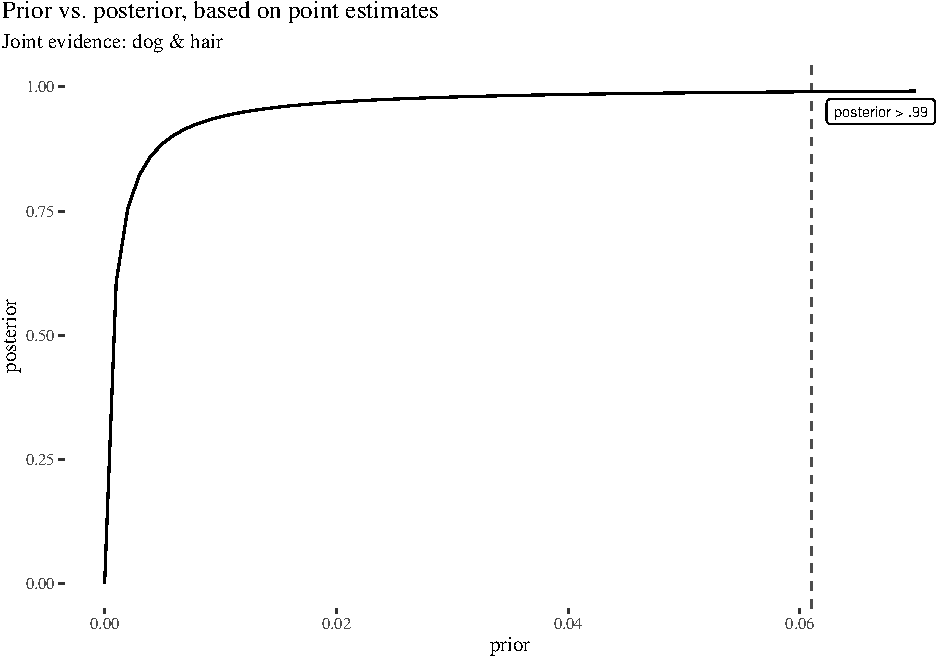
\includegraphics[width=0.6\linewidth]{paper-outline_files/figure-latex/impactOfPoint4-1} \end{center}
\caption{Impact of dog fur and human hair evidence on the prior, point estimates.}
\label{fig:impactOfPoint}
\end{figure}

Unfortunately, this analysis leaves out something crucial. You reflect
on what you have been told and ask the expert: how can you know the
random match probabilities with such precision? Shouldn't we also be
mindful of the uncertainty that may affect these numbers? The expert
agrees, and tells you that in fact the random match probability for the
hair evidence is based on 29 matches found in a database of size 1148,
while the random match probability for the dog evidence is based on
finding two matches in a reference database of size 78.

The expert's answer makes apparent that the precise random match
probabilities do not tell the whole story. Perhaps, the information
about sample sizes is good enough and now you know how to use the
evidence properly.\footnote{This is what, effectively, CITE TARONI seem
  to suggest when they insist the fact-finders should be simply given
  point estimates and information about the study set-up, such as sample
  size. As will transpire, we disagree.} But if you are like most human
beings, you can't. What to do, then?\\
\todo{added this bit to draw attention to this aspect of the Taroni debate, to come back to this}

You ask the expert for guidance: what are reasonable ranges of the
random match probabilities? What are the worst-case and best-case
scenarios? The expert responds with 99\% credible
intervals---specifically, starting with uniform priors, the ranges of
the random match probabilities are (.015,.037) for hair evidence and
(.002, .103) for fur evidence.\footnote{Roughly, the 99\% credible
  interval is the narrowest interval to which the expert thinks the true
  parameter belongs with probability .99. For a discussion of what
  credible intervals are, how they differ from confidence intervals, and
  why confidence intervals should not be used, see Chapter 3.} With this
information, you redo your calculations using the upper bounds of the
two intervals: \(.037\) and \(.103\). The rationale for choosing the
upper bounds is that these numbers result in random match probabilities
that are most favorable to the defendant. Your new calculation yields
the following: \begin{align*}
\mathsf{P}(\s{dog}\wedge \s{hair} \vert \neg \s{source})   & =  .037 \times .103 =.003811.
\end{align*} This number is around 5.88 times greater than the original
estimate. Now the prior probability of the source hypothesis needs to be
higher than 0.274 for the posterior probability to be above .99 (Figure
\ref{fig:impactOfCharitable}). So you are no longer convinced that the
two items of match evidence are strongly incriminating.

\begin{figure}[H]

\begin{center}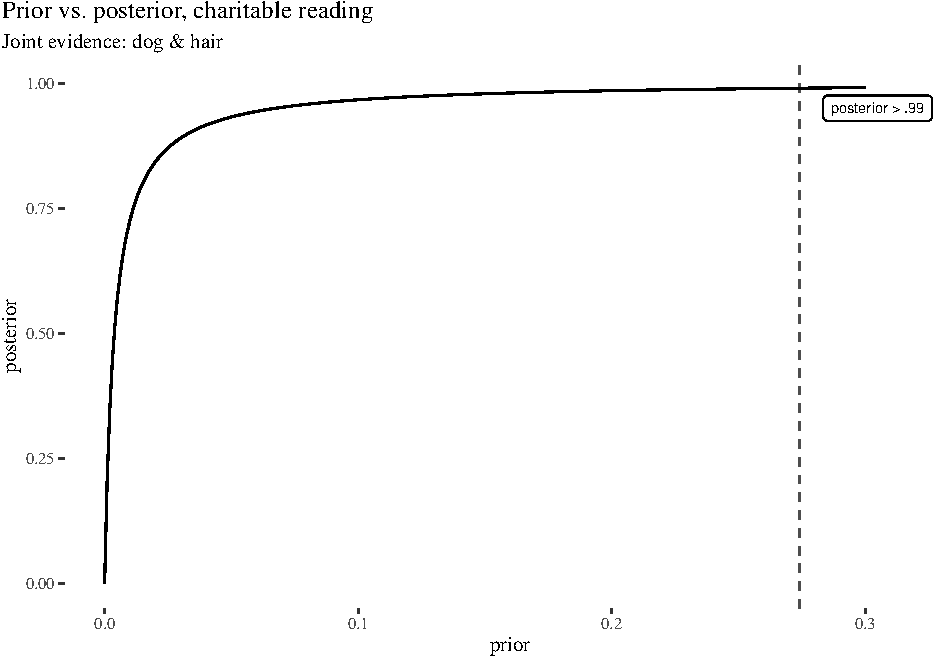
\includegraphics[width=0.6\linewidth]{paper-outline_files/figure-latex/fig:charitableImpact7-1} \end{center}
\caption{Impact of dog fur and human hair evidence on the prior, charitable reading.}
\label{fig:impactOfCharitable}
\end{figure}

This result is puzzling. Are the two items of match evidence strongly
incriminating evidence (as you initially thought) or somewhat weaker (as
the new calculation suggests)? For one thing, using precise random match
probabilities might be too unfavorable toward the defendant. On the
other hand, your new assessment of the evidence based on the upper
bounds might be too \emph{favorable} toward them. Is there a middle way
that avoids overestimating and underestimating the strength of the
evidence?

To see what this middle path looks like, we should reconsider the
calculations you just did. You made an important blunder: you assumed
that because the worst-case probability for one event is \(x\) and the
worst-case probability for another independent event is \(y\), the
worst-case probability for their conjunction is \(xy\). But this
conclusion does not follow if the margin of error (credible interval) is
fixed. The intuitive reason is simple: just because the probability of
an extreme (or larger absolute) value \(x\) for one variable \(X\) is
.01, and so it is for the value \(y\) of another independent variable
\(Y\), it does not follow that the probability that those two
independent variables take values \(x\) and \(y\) simultaneously is the
same. This probability is actually much smaller. The interval
presentation instead of doing us good led us into error.

In general, it is impossible to calculate the credible interval for the
joint distribution based solely on the individual credible intervals
corresponding to the individual events. We need additional information:
the distributions that were used to calculate the intervals for the
probabilities of the individual events. In our example, if you
additionally knew, for instance, that the expert used beta distributions
(as, arguably, they should in this context), you could in principle
calculate the 99\% credible interval for the joint distribution. It
usually will not be the same as whatever the results of multiplication
of individual interval edges, and it is unlikely that a human
fact-finder would be able to correctly run such calculations in their
head even if they knew the functional form of the distributions used.
\footnote{Also, in principle, in more complex contexts, we need further
  information about how the items of evidence are related if we cannot
  take them to be independent.} So providing the fact-finder with
individual intervals, even if further information about the
distributions is provided, might easily mislead.\footnote{Investigation
  of the extent to which the individual interval presentation is
  misleading would be an interesting psychological study.}
\todo{Can you google to see if there is any such study?}

As it turns out, given the reported sample sizes, the 99\% credible
interval for the probability
\(\mathsf{P}(\s{dog}\wedge \s{hair} \vert \neg \s{source})\) is
\((0.000023, 0.002760)\). \todo{the fn was repetitive, compare to fn 5}

The upper bound of this interval would then require the prior
probability of the source hypothesis to be above .215 for the posterior
to be above .99. On this interpretation, the two items of match evidence
are still not quite as strong as you initially thought, but stronger
than what your second calculation indicated.

Still, the interval approach---even the corrected version just
outlined---suffers from a more general problem. Working with intervals
might be useful if the underlying distributions are fairly symmetrical.
But in our case, they might not be. For instance, Figure
\ref{fig:densities} depicts beta densities for dog fur and human hair,
together with sampling-approximated density for the joint evidence. The
distribution for the joint evidence is not symmetric. If you were only
informed about the edges of the interval, you would be oblivious to the
fact that the most likely value (and the bulk of the distribution,
really) does not simply lie in the middle between the edges. Just
because the parameter lies in an interval with some posterior
probability, it does not mean that the ranges near the edges of the
interval are equally likely---the bulk of the density might very well be
closer to one of the edges. Therefore, only relying on the edges can
lead one to either overestimate or underestimate the probabilities at
play. This also means that---following our advice on how to illustrate
the impact of evidence on prior probabilities---a better representation
of the dependence of the posterior on the prior should comprise multiple
possible sampled lines whose density mirrors the density around the
probability of the evidence (Figure \ref{fig:lines}).

\begin{figure}[H]

\begin{center}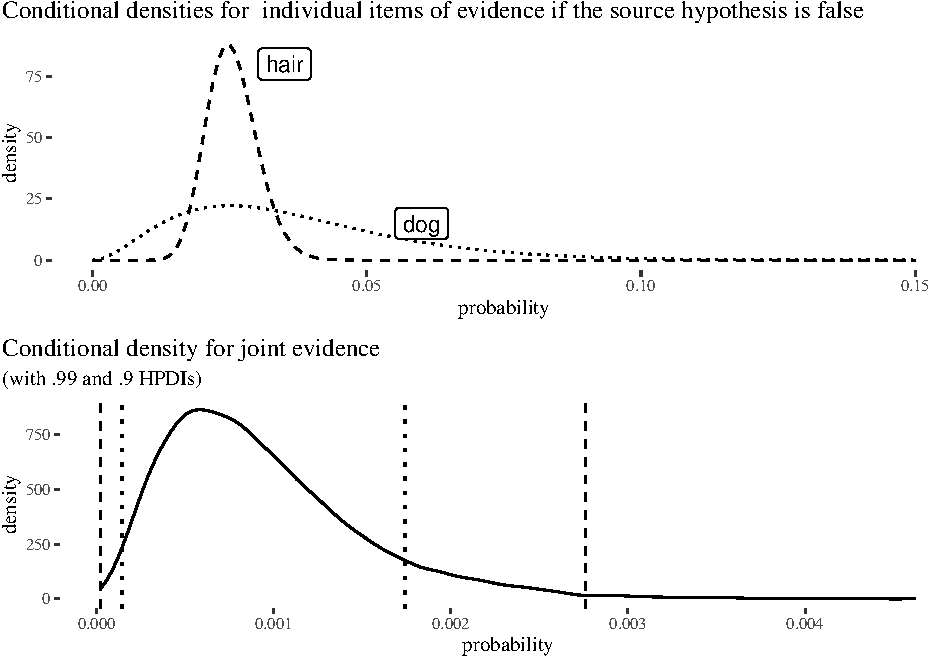
\includegraphics[width=0.8\linewidth]{paper-outline_files/figure-latex/fig:densities-1} \end{center}
\caption{Beta densities for individual items of evidence and the resulting joint density with .99 and .9 highest posterior density intervals, assuming the sample sizes as discussed and independence, with uniform priors.}
\label{fig:densities}
\end{figure}

\hypertarget{references}{%
\section*{References}\label{references}}
\addcontentsline{toc}{section}{References}

\hypertarget{refs}{}
\begin{CSLReferences}{1}{0}
\leavevmode\vadjust pre{\hypertarget{ref-deadman1984fiber2}{}}%
Deadman, H. A. (1984a). Fiber evidence and the wayne williams trial
(conclusion). \emph{FBI L. Enforcement Bull.}, \emph{53}, 10--19.

\leavevmode\vadjust pre{\hypertarget{ref-deadman1984fiber1}{}}%
Deadman, H. A. (1984b). Fiber evidence and the wayne williams trial
(part i). \emph{FBI L. Enforcement Bull.}, \emph{53}, 12--20.

\end{CSLReferences}

\end{document}
